\section{Ponte di Wien invertito come filtro notch}
\subsection{Acquisizione dati}
Utilizzando un ponte di Wien ``invertito'' è possibile creare un filtro notch. Esso non è efficace come quello montato nell'esperienza precedente ma è tuttavia interessante in quanto entrambi i capi del circuito contribuiscono alla creazione del segnale finale. Come si vede in Fig. \ref{fig:Winv} sia $V_1$ che $V_2$ sono variabili nel tempo. Un'implicazione di ciò è che un eventuale circuito collegato al ponte di Wien non può essere messo a terra (per questo non è stato possibile eseguire direttamente una misura della differenza di potenziale tra i capi attraverso l'oscilloscopio, il quale è per struttura messo a terra).
\begin{wrapfigure}[15]{r}[0pt]{80mm}
	\centering
    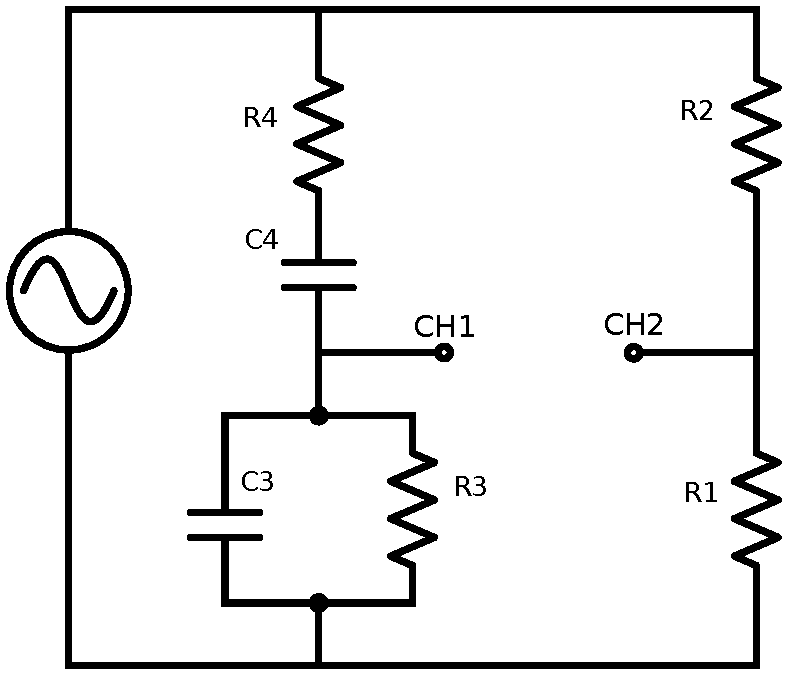
\includegraphics[width=0.30\textwidth]{schema2.pdf}
    \caption{Schema del ponte di Wien invertito}
    \label{fig:Winv}
\end{wrapfigure}

\subsection{analisi dati}